\def\duedate{\today}
\def\HWnum{5}
\documentclass[10pt,a4paper]{book}

% custom section formatting
\usepackage{titlesec}
\titleformat{\chapter}[display]
{\normalfont\Large\filcenter\sffamily}
{\titlerule[1pt]%
\vspace{1pt}%
\titlerule
\vspace{1pc}%
\LARGE\MakeUppercase{\chaptertitlename} \thechapter}
{1pc}
{\titlerule
\vspace{1pc}%
\Huge}

% appendix handling
\usepackage[toc,page]{appendix}
    
% encoding for file and font
\usepackage[utf8]{inputenc}
\usepackage[T1]{fontenc}

% math formatting/tools
\usepackage{amsmath}
\usepackage{amssymb}
\usepackage{mathtools}
\usepackage[arrowdel]{physics}

% unit formatting
\usepackage{siunitx}
\AtBeginDocument{\RenewCommandCopy\qty\SI}

% figure formatting/tools
\usepackage{graphicx}
\usepackage{float}
\usepackage{subcaption}
\usepackage{multirow}
\usepackage{import}
\usepackage{pdfpages}
\usepackage{transparent}
\usepackage{currfile}

\NewDocumentCommand\incfig{O{1} m}{
    \def\svgwidth{#1\textwidth}
    \import{./Figures/\currfiledir}{#2.pdf_tex}
}

\newcommand{\bef}{\begin{figure}[h!tb]\centering}
\newcommand{\eef}{\end{figure}}

\newcommand{\bet}{\begin{table}[h!tb]\centering}
\newcommand{\eet}{\end{table}}

% hyperlink references 
\usepackage{hyperref}
\hypersetup{
    colorlinks=true,
    linkcolor=blue,
    filecolor=magenta,
    urlcolor=cyan,
    pdftitle={Physics 1 Notes},
    pdfauthor={Richard Whitehill},
    pdfpagemode=FullScreen
}
\urlstyle{same}

\newcommand{\eref}[1]{Eq.~(\ref{eq:#1})}
\newcommand{\erefs}[2]{Eqs.~(\ref{eq:#1})--(\ref{eq:#2})}

\newcommand{\fref}[1]{Fig.~(\ref{fig:#1})}
\newcommand{\frefs}[2]{Fig.~(\ref{fig:#1})--(\ref{fig:#2})}

\newcommand{\aref}[1]{Appendix~(\ref{app:#1})}
\newcommand{\sref}[1]{Section~(\ref{sec:#1})}
\newcommand{\srefs}[2]{Sections~(\ref{sec:#1})-(\ref{sec:#2})}

\newcommand{\tref}[1]{Table~(\ref{tab:#1})}
\newcommand{\trefs}[2]{Table~(\ref{tab:#1})--(\ref{tab:#2})}

% tcolorbox formatting/definitions
\usepackage[most]{tcolorbox}
\usepackage{xcolor}
\usepackage{xifthen}
\usepackage{parskip}

\definecolor{peach}{rgb}{1.0,0.8,0.64}

\DeclareTColorBox[auto counter, number within=chapter]{defbox}{O{}}{
    enhanced,
    boxrule=0pt,
    frame hidden,
    borderline west={4pt}{0pt}{green!50!black},
    colback=green!5,
    before upper=\textbf{Definition \thetcbcounter \ifthenelse{\isempty{#1}}{}{: #1} \\ },
    sharp corners
}

\newcommand*{\eqbox}{\tcboxmath[
    enhanced,
    colback=black!10!white,
    colframe=black,
    sharp corners,
    size=fbox,
    boxsep=8pt,
    boxrule=1pt
]}

\newtcolorbox[auto counter, number within=chapter]{exbox}{
    parbox=false,
    breakable,
    enhanced,
    sharp corners,
    boxrule=1pt,
    colback=white,
    colframe=black,
    before upper= \textbf{Example \thetcbcounter:}\,,
    before lower= \textbf{Solution:}\,,
    segmentation hidden
}

\newtcolorbox{resbox}{
    enhanced,
    colback=black!10!white,
    colframe=black,
    boxrule=1pt,
    boxsep=0pt,
    top=2pt,
    ams nodisplayskip,
    sharp corners
}


\begin{document}

\prob{1}{

(a) Two halves of a long hollow conducting cylinder of inner radius $b$ are separated by small lengthwise gaps on each side, and are kept at different potentials $V_1$ and $V_2$.
Show that the potential inside is given by 
\begin{eqnarray}
    \Phi(s,\phi) = \frac{V_1 + V_2}{2} + \frac{V_1 - V_2}{\pi} \arctan(\frac{2 b s}{b^2 - s^2} \cos{\phi})
,\end{eqnarray}
where $\phi$ is measured from a plane perpendicular to the plane through the gap.

(b) Calculate the surface-charge density on each half of the cylinder.

}

\sol{

In polar coordinates with translational symmetry along the $z$ axis, Laplace's equation reads
\begin{eqnarray}
    \laplacian \Phi = \frac{1}{s} \pdv{s} \Big( s \pdv{\Phi}{s} \Big) + \frac{1}{s^2} \pdv[]{\Phi}{s}
.\end{eqnarray}
We can guess an ansatz for a particular solution as
\begin{eqnarray}
    \Phi(s,\phi) = R(s) T(\phi)
,\end{eqnarray}
which gives two separate second-order ordinary differential equations for the $s$ and $\phi$ dependence:
\begin{gather}
    s \dv{s}\Big( s \dv{R}{s} \Big) - \nu^2 R = 0 \\
    \dv[2]{T}{\phi} + \nu^2 T = 0
.\end{gather}
Note that we have written these equations choosing the sign of $\nu^2$ with the foresight that $T$ must be cyclic (i.e. $T(\phi + 2\pi) = T(\phi)$).
Thus, we can write the general solution
\begin{eqnarray}
    \Phi(s,\phi) = (a_0 + b_0 \ln{s})(A_0 + B_0 \phi) + \sum_{\nu > 0} (a_{\nu} s^{\nu} + b_{\nu} s^{-\nu}) (A_{\nu} \cos{\nu \phi} + B_{\nu} \sin{\nu \phi})
.\end{eqnarray}
Since we are interested in $\Phi$ in the region $s \leq b$, we must have $b_0 = b_{\nu} = 0$ such that $\Phi$ is finite.
Let us then write
\begin{eqnarray}
    \Phi(s,\phi) = A_0 + B_0 \phi + \sum_{\nu > 0} [A_{\nu} \cos{\nu \phi} + B_{\nu} \sin{\nu \phi} ] s^{\nu}
,\end{eqnarray}
where we have absorbed the constants $a_{\nu}$ into $A_{\nu}$ and $B_{\nu}$.
Note that since $\Phi(s,\phi + 2\pi) = \Phi(s,\phi)$, we must have $B_0 = 0$ and $\nu = n \in \naturals$\footnote{Equating $\Phi(s,\phi+2\pi)$ and $\Phi(s,\phi)$, we get the equations $2\pi B_0 = 0$, $\cos(2\pi\nu) + \sin(2\pi\nu) = 1$, and $\cos(2\pi\nu) - \sin(2\pi\nu) = 1$, which reduces to $\sin(2\pi\nu) = 0$ and $\cos(2\pi\nu) = 1$ which are only satisfied if $2\pi\nu = 2 \pi n$ or $\nu = n$.}, which leaves us with
\begin{eqnarray}
    \Phi(s,\phi) = A_0 + \sum_{n=1}^{\infty} [A_{n} \cos(n\phi) + B_{n} \sin(n\phi)] s^{n}
.\end{eqnarray}
We can solve for the $A_{n}$ and $B_{n}$ using the orthogonality relations (for $n > 0$)
\begin{align}
    \int_{-\pi}^{\pi} \sin(mx)\sin(nx) \dd{x} &= \pi \delta_{nm} \\
    \int_{-\pi}^{\pi} \sin(mx)\cos(nx) \dd{x} &= 0 \\
    \int_{-\pi}^{\pi} \cos(mx)\cos(nx) \dd{x} &= \pi \delta_{nm}
,\end{align}
where $\delta_{nm}$ is the kronecker-delta symbol.
Hence,
\begin{align}
    A_0 &= \frac{1}{2\pi} \int_{-\pi}^{\pi} \Phi(b,\phi) \dd{\phi} = \frac{V_1 + V_2}{2} \\
    A_{n>0} &= \frac{1}{\pi b^{n}} \int_{-\pi}^{\pi} \Phi(b,\phi) \cos(n\phi) \dd{\phi} = 0 \\
    B_{n>0} &= \frac{1}{\pi b^{n}} \int_{-\pi}^{\pi} \Phi(b,\phi) \sin(n\phi) \dd{\phi} = \frac{1}{\pi b^{n}} \frac{V_1 - V_2}{n} [1 - (-1)^{n}]
.\end{align}
Putting this into the expression for $\Phi$, we arrive at
\begin{eqnarray}
    \Phi(s,\phi) = \frac{V_1 + V_2}{2} + \frac{V_1 - V_2}{\pi} \Bigg[ 2 \sum_{n=0}^{\infty} \frac{\sin[(2n+1)\phi]}{n} \Big( \frac{s}{b} \Big)^{2n+1} \Bigg]
.\end{eqnarray}

Finally, we only have to find the value of the series in the second term.
We do so by writing
\begin{eqnarray}
    S = 2\sum_{n=0}^{\infty} \frac{\sin[(2n+1) \phi]}{n} \Big( \frac{s}{b} \Big)^{2n+1} = \Im{ 2\sum_{n=0}^{\infty} \frac{1}{n} \Big( \frac{s}{b} e^{i\phi} \Big)^{2n+1} } \\
.\end{eqnarray}
Recall that
\begin{align}
    \ln(1 + x) &= \sum_{n=0}^{\infty} \frac{(-1)^{n+1}}{n} x^{n} = -\sum_{n=0}^{\infty} \frac{x^{2n}}{2n} + \sum_{n=0}^{\infty} \frac{x^{2n+1}}{2n+1} \\
    \ln(1 - x) &= \sum_{n=0}^{\infty} \frac{(-1)^{n+1}}{n} (-1)^{n} x^{n} = -\sum_{n=0}^{\infty} \frac{x^{2n}}{2n} - \sum_{n=0}^{\infty} \frac{x^{2n+1}}{2n+1} \\
    &\Rightarrow \ln(1 + x) - \ln(1 - x) =\ln( \frac{1 + x}{1-x} ) = 2 \sum_{n=0}^{\infty} \frac{x^{2n+1}}{2n + 1}
,\end{align}
and therefore, we can write\footnote{Notice that $(b+s e^{i\phi})(b - s e^{-i\phi}) = (b^2 - s^2) + 2i b s \sin{\phi}$.}
\begin{eqnarray}
    S = \Im{ \ln( \frac{1 + (s/b)e^{i\phi}}{1 - (s/b)e^{i\phi}} ) } = \arctan\Bigg[ \frac{2 s b \sin{\phi}}{b^2 - s^2} \Bigg]
.\end{eqnarray}

We then arrive at the final result
\begin{eqnarray}
    \eqbox{ \Phi(s,\phi) = \frac{V_1 + V_2}{2} + \frac{V_1 - V_2}{\pi} \arctan( \frac{2bs \sin{\phi}}{b^2 - s^2} ) }
.\end{eqnarray}

(b) The surface charge density on each half of the sphere is given by
\begin{eqnarray}
\eqbox{
\begin{aligned}
    \sigma &= \epsilon_0 \pdv{\Phi}{s} \Big|_{s = b} = \epsilon_0 \frac{V_1 - V_2}{\pi} \frac{(b^2 - s^2)^2}{(b^2 - s^2)^2 + 4 b^2 s^2 \sin^2{\phi}} \frac{2b(b^2 + s^2)}{(b^2 - s^2)^2} \sin{\phi} \Big|_{s = b} \\
    &= \frac{\epsilon_0 (V_1 - V_2)}{\pi b \sin{\phi}}
.\end{aligned}
    }
\end{eqnarray}
Observe that if $\phi \in [-\pi,0]$ that $\sigma \sim V_2 - V_1$, while on $[0,\pi]$ $\sigma \sim V_1 - V_2$, meaning that points on the cylinder reflected about the plane splitting the cylinder have surface charge densities of opposite sign but the same magnitude.
}


\prob{2}{

    A variant of the preceding two-dimensional problem is a long hollow conducting cylinder of radius $b$ that is divided into equal quarters, alternate segments being held at potential $+V$ and $-V$. \\[1pt]

(a) Solve by means of the series solution [See Eq. (2.71) in \textit{Jackson} and Eq. (13.5.9) in Lecture 10] and show that the potential inside the cylinder is
\begin{eqnarray}
    \Phi(s,\phi) = \frac{4V}{\pi} \sum_{n=0}^{\infty} \Big( \frac{s}{b} \Big)^{4n+2} \frac{\sin[(4n+2)\phi]}{2n+1}
.\end{eqnarray}

(b) Sum the series and show that
\begin{eqnarray}
    \Phi(s,\phi) = \frac{2V}{\pi} \arctan(\frac{2 s^2 b^2 \sin{2\phi}}{b^{4} - s^{4}})
.\end{eqnarray}

(c) Sketch the field lines and equipotentials.

}

\sol{

(a) We wrote down the generic solution for a setup such as this
\begin{eqnarray}
    \Phi(s,\phi) = A_0 + \sum_{n=1}^{\infty} [ A_{n}\cos(n\phi) + B_{n}\sin(n\phi) ] \Big( \frac{s}{b} \Big)^{n}
.\end{eqnarray}
Note that we have redefined our constants, anticipating that these factors will show up when we use the orthogonality relations: $A_{n} \rightarrow A_{n}/b^{n}$ and $B_{n} \rightarrow B_{n}/b^{n}$.
The constants are determined in the same way as in problem (1):
\begin{align}
    A_{0} &= \frac{1}{2\pi} \int_{-\pi}^{\pi} \Phi(b,\phi) \dd{\phi} = 0 \\
    A_{n > 0} &= \frac{1}{\pi} \int_{-\pi}^{\pi} \Phi(b,\phi) \cos(n\phi) \dd{\phi} = 0 \\
    B_{n > 0} &= \frac{1}{\pi} \int_{-\pi}^{\pi} \Phi(b,\phi) \sin(n\phi) \dd{\phi} = \frac{V}{\pi n} [ 1 - (-1)^{n} - 2\cos(\pi n /2) ]
,\end{align}
defining 
\begin{eqnarray}
    \Phi(b,\phi) = \begin{cases}
        +V & \phi \in (0,\pi/2) \cup (-\pi,-\pi/2) \\
        -V & \phi \in (\pi/2,\pi) \cup (-\pi/2,0) \\
    \end{cases}
.\end{eqnarray}
Note that the coefficients $B_{n}$ require a little more care this time.
We will write $n = 4k + r$, where $k \in \integers$ and $r \in \{ 0,1,2,3 \} $, which gives
\begin{eqnarray}
    B_{n} = \frac{2V}{\pi n} [1 + (-1)^{r} - 2 \cos(r \pi / 2)] = \frac{2V}{\pi n} \begin{cases}
        0 & r = 0 \\
        0 & r = 1 \\
        4 & r = 2 \\
        0 & r = 3
    \end{cases}
.\end{eqnarray}
Therefore, the series becomes
\begin{eqnarray}
    \eqbox{ \Phi(s,\phi) = \frac{4 V}{\pi} \sum_{n=0}^{\infty} \frac{\sin[(4n + 2) \phi]}{2n+1} \Big( \frac{s}{b} \Big)^{4n + 2} }
.\end{eqnarray}

(b) We can use the result of problem (1), taking $x \rightarrow x^2$, which gives
\begin{eqnarray}
    \ln(\frac{1 + x^2}{1 - x^2}) = 2 \sum_{n=0}^{\infty} \frac{x^{4n +2}}{2n+1}
\end{eqnarray}
and
\begin{eqnarray}
    2 \sum_{n=0}^{\infty} \frac{\sin[(4n+2)\phi]}{2n + 1} \Big( \frac{s}{b} \Big)^{4n+2} = \Im{ \ln(\frac{b^2 + s^2e^{2i\phi}}{b^2 - s^2 e^{2i\phi}}) } = \arctan( \frac{2b^2 s^2 \sin{2\phi}}{b^{4} - s^{4}} )
.\end{eqnarray}

Thus, we arrive at
\begin{eqnarray}
    \eqbox{ \Phi(s,\phi) = \frac{2 V}{\pi} \arctan( \frac{2b^2s^2 \sin{2\phi}}{b^{4} - s^{4}} ) }
.\end{eqnarray}

(c) If we write $s = b\xi$ and $x = \cos{\phi}$, $y = \sin{\phi}$, then the equipotential lines are given by
\begin{eqnarray}
    \label{eq:lcurves}
    \frac{4 x y (x^2 + y^2)}{1 - (x^2 + y^2)^2} = \tan(\frac{\pi}{2} \frac{\Phi}{V})
.\end{eqnarray}
Notice that $|\Phi| \leq V$ since $|\arctan{x}| \leq \pi/2$.
A plot of selected level curves is shown in \fref{prob2c-1}.

\begin{figure}[h!]
    \centering
    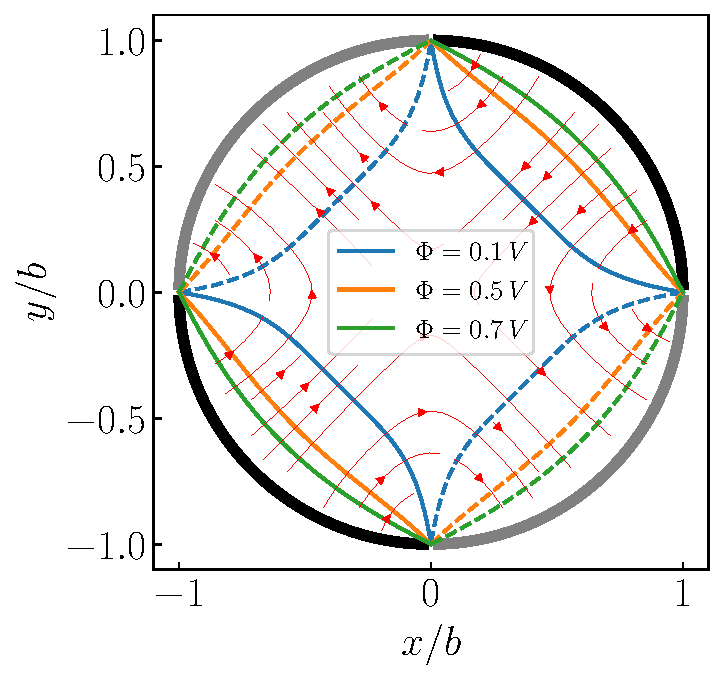
\includegraphics[width=0.5\textwidth]{prob2c-1.pdf}
    \caption{Plot of level curves satisfying \eref{lcurves} for a selection of $\Phi/V$, where the black and gray lines represent the portions of the cylinder held at potentials $\pm V$, respectively. Note that the solid lines are for $\Phi > 0$, while the dashed lines are the corresponding curves with $\Phi < 0$. The electric field lines are also imposed on the plot. Observe that the field lines are always perpendicular to the equipotential lines, and furthermore, they point from the positive}
    \label{fig:prob2c-1}
\end{figure}

}


\prob{3}{

A hollow cube has conducting walls defined by six planes $x = 0$, $y = 0$, $z = 0$ and $x = a$, $y=a$, $z = a$.
The walls $z = 0$ and $z = a$ are held at a constant potential $V$.
The other four sides are at zero potential. \\[1pt]

(a) Find the potential $\Phi(x,y,z)$ at any point inside the cube.

(b) Evaluate the potential at the center of the cube numerically, accurate to three significant figures.
How many terms in the series is it necessary to keep in order to attain this accuracy?
Compare your numerical result with the average value of the potential on the walls.

(c) Find the surface-charge density on the surface $z = a$.

}

\sol{}


\prob{4}{

The two-dimensional region, $s \geq a$, $0 \leq \phi \leq \beta$ is bounded by conducting surfaces at $\phi = 0$, $s = a$, and $\phi = \beta$ held at zero potential, as indicated in the sketch.
At large $s$ the potential is determined by some configuration of charges and/or conductors at fixed potentials.

(a) Write down a solution for the potential $\Phi(s,\phi)$ that satisfies the boundary conditions for finite $s$.

(b) Keeping only the lowest nonvanishing terms, calculate the electric field components $E_{s}$ and $E_{\phi}$ and also the surface-charge densities $\sigma(s,0)$, $\sigma(s,\beta)$, and $\sigma(a,\phi)$ on the three boundary surfaces.

(c) Consider $\beta = \pi$ (a plane conductor with a half cylinder of radius $a$ on it).
Show that far from the half-cylinder the lowest order terms of part (b) give a uniform electric field normal to the plane.
Sketch the charge density on and in the neighborhood of the half-cylinder.
For fixed electric field strength far from the plane, show that the total charge on the half-cylinder (actually charge per unit length in the $z$ direction) is twice as large as would reside on a strip of width $2a$ in its absence.
Show that the extra portion is drawn from regions on the plane nearby, so that the total charge on a strip of width large compared to $a$ is the same whether the half-cylinder is there or not.

}

\sol{}




\end{document}
